\documentclass[a4paper, 11pt, twocolumn]{report}
\usepackage[
	backend=biber,
	natbib=true,
	style=numeric,
	sorting=none
]{biblatex}
\addbibresource{report.bib}
\usepackage{authblk}
\usepackage[left=0.7in, right=0.7in, top=0.7in, bottom=0.9in]{geometry}
\usepackage{listings}
\usepackage{appendix}
\usepackage{graphicx}
\usepackage{bm}
\usepackage{array}
\usepackage{mathtools}
\usepackage{amssymb}
\usepackage{wrapfig}
\usepackage{listings}
\usepackage{tabulary}
\usepackage{algorithm}
\usepackage{algpseudocode}
\usepackage{algorithmicx}
\usepackage[font=small,skip=2pt]{caption}
\hyphenpenalty=10000
\linespread{1.03}
\setlength{\columnsep}{0.25in}
\renewcommand{\thesection}{\arabic{section}}

\begin{document}
\lstset{language=Matlab, basicstyle=\small}
\title{\textbf{COMP6208 Advanced Machine Learning} \\
{\Large Student Mini-Projects}}

\author{\textbf{Alexander Ally} (aa2g11)\\
\textbf{Hendrik Appel} (hja1g11)\\
\textbf{Samir Moussa} (sm28g11)}

\affil{School of Electronics and Computer Science\\
Faculty of Physical Sciences and Engineering\\
University of Southampton}
\date{Thursday 7\textsuperscript{th} May 2015}
\maketitle

\begin{abstract}

This is a report describing the preprocessing methods, machine learning algorithms and validation techniques used to find a solution to a typical real-world machine learning problem in the driver telematics analysis space.
The task is to model individual drivers based on their driving behaviour specified by their trip data to identify whether a particular trip has been driven by a driver or otherwise.
Several approaches were studied and utilised to find a practical solution to a challenging task and our experiments are detailed in this report.
We found that ensemble tree-based methods and deep belief networks performed fairly well at classifying trips.

\end{abstract}

% section
\section{Introduction}





% section
\section{Problem Scenario}

The task detailed in this report is to use telematic data to identify driver signatures.
This problem was initially released as a challenge available to members of the machine learning community provided by Kaggle\footnote{kaggle.com/c/axa-driver-telematics-analysis} and supported by multinational insurance company AXA.
For automobile insurers, understanding the driving behaviour (telematics) of their customers allows them to quantify liability and price their insurance policies according to the risk associated with different drivers.
For drivers, policies can be better suited to their experience and driving mannerisms.
The end task is to develop an algorithmic signature or ``telematic fingerprint" of a driver to identify when a particular trip has been driven by that driver.

Deciding to solve this machine learning problem was due to the appeal of facing challenges and complexities involved in dealing with real-world information and being able to apply machine learning methods to extract useful information and make sense of it.
As demonstrated throughout the report, obstacles were far from few.

\subsection{Dataset}

The AXA dataset contains over 2,700 drivers and each driver has 200 trips associated.
Each trip is specified by a variable-length list of $(x,y)$ coordinates describing the position of the driver at each second relative to the starting position.
To protect the privacy of drivers and their information, all trips are centred to start at the origin $(0,0)$, randomly rotated and partially truncated from either the beginning or end of the trip.
A typical set of 200 trips for a driver are plotted in figure \ref{fig:tripsgraph}.
False trips are assigned to each driver and but it is not possible to distinguish between true positive and true negative trips due to the absence of labels.
The size of the entire dataset is just over half a terabyte with exactly 547,200 trips to predict.

\begin{figure}[h]
    \center
    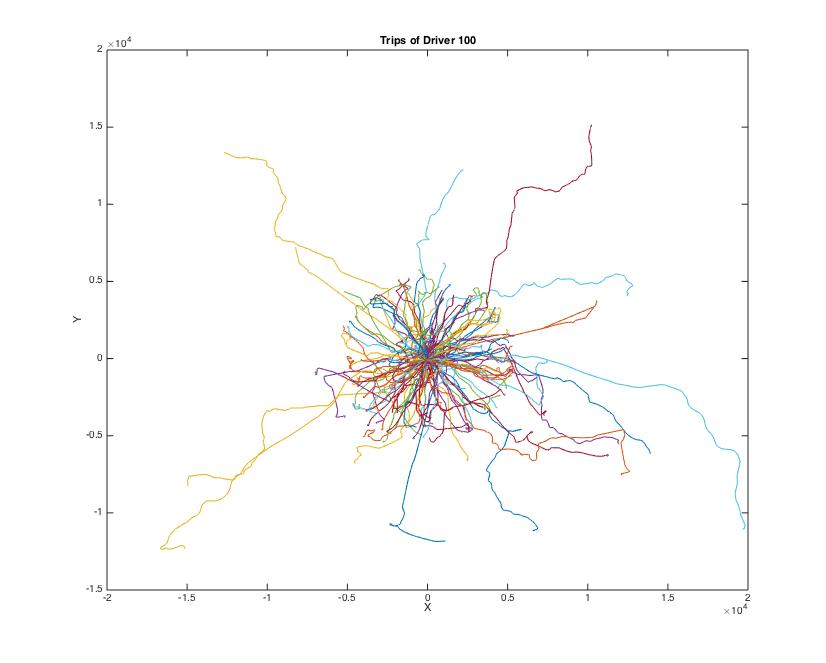
\includegraphics[width=\linewidth]{sample_driver_vis}
    \caption{Typical illustration of trips for a driver.}
    \label{fig:tripsgraph}
\end{figure}


\subsection{Challenges}

As expected with most real-world data, there were a variety of challenges that needed to be overcome in order to start experimentation.
The challenges faced, specifically with this problem, was the unavailability of labels, presenting us with an unsupervised learning problem.
Our models therefore needed to consider learning latent variables or take on clustering methods to try and find some structure to the data.
Moreover, the fact that coordinates do not offer any useful description, some preprocessing and feature extraction was required.
The features may be extracted manually using prior knowledge of the problem domain or learned though hidden variables as in neural networks.

Since the dataset is very large, it was expected to take a fairly long time to perform preprocessing and learn a model.
To overcome this, some parallelisation work was required, utilising the university's available computing power.
Finally, the data included some degree of noise and missing values due to the inaccuracies associated with GPS readings.
Although little feedback was expected to be given from our models in terms of validating the accuracy of our predictions, a submission to the Kaggle competition did present us with an overall score, although this did not give us information of any use to improve our models.




\subsection{Variant Approaches}






% section
\section{Analysis \& Experimentation}

\subsection{Preprocessing}

Forming useful features from unstructured data allows learning algorithms to perform well while minimising the amount of redundant data.
A system named \textit{representation learning} requires a model to not only learn a mapping function from input to output, but intrinsically learn a representation of the data within the model.
As discussed later, unsupervised learning techniques, particularly deep learning, aim to apply representation learning to establish a expressive representation of the underlying data, enough to extract useful information and reason about new information.

Since the raw data is unstructured and does not provide useful, or in fact any description of the important underlying features surrounding that of a driver and their driving behaviour, much of the complications faced throughout the project arose from the extraction of effective features.
The trips were merely composed of sequences of GPS coordinates taken at one-second intervals.
The data had to be processed and features were to be designed before machine learning techniques could be applied to make predictions.
In addition the GPS coordinates given in the data were subject to inaccuracy.

The extracted features contained $N_F$ continuous variables and can be summarised by the list in appendix X.


\subsection{Data Smoothing}
Because the features were often based upon first and second order gradients of the original data, noise caused a lot of problems.
Particularly when the speed of the vehicle was low, small fluctuations in the position of the vehicle caused a small velocity and acceleration to be reported.
When directional information is extracted from these gradients (and magnitude information thrown away) there would appear to be wild changes in direction when really the vehicle was stationary and there was small fluctuations in the position information being reported.

In order to solve this problem a number of different avenues were explored.
One simple approach was report any velocity with a magnitude of less than a small value to be set to 0.
However this ignored smoothness issues that occurred at higher speeds.
To remedy this a simple filter was constructed by applying the Discrete Fourier Transform and reconstructing th data using fewer components.
This does appear to work well in general but in sections where the driver is crawling along at a very low speed were the filter wrongly assumes that the driver is stationary.
This can be observed in the plot in figure \ref{fig:fouriersmooth}.

\begin{figure}[h]
    \center
    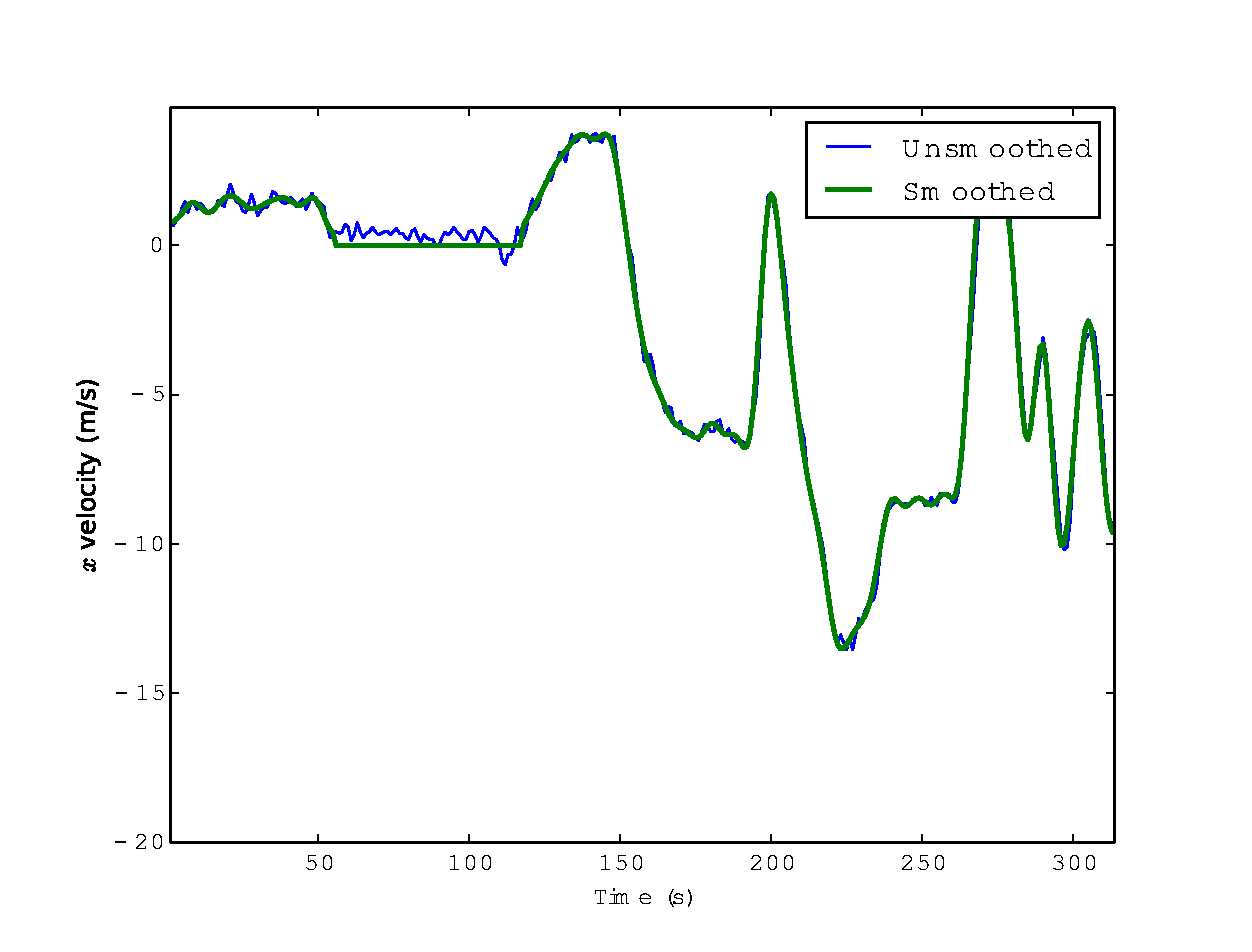
\includegraphics[width=\linewidth]{fouriersmooth}
    \caption{Fourier smoothed velocity component.}
    \label{fig:fouriersmooth}
\end{figure}

Another approach attempted was to apply the Savitzky-Golay filter to smooth the data.
Savitzky-Golay smooths data by convolution, fitting a polynomial to successive windows over the data points using a least squares optimisation.
One can see that in figure \ref{fig:savgolsmooth} that the problem of threshold smoothing is does not appear and that the data appears to be much smoother.
However some jaggedness remains in periods of low velocity.

\begin{figure}[h]
    \center
    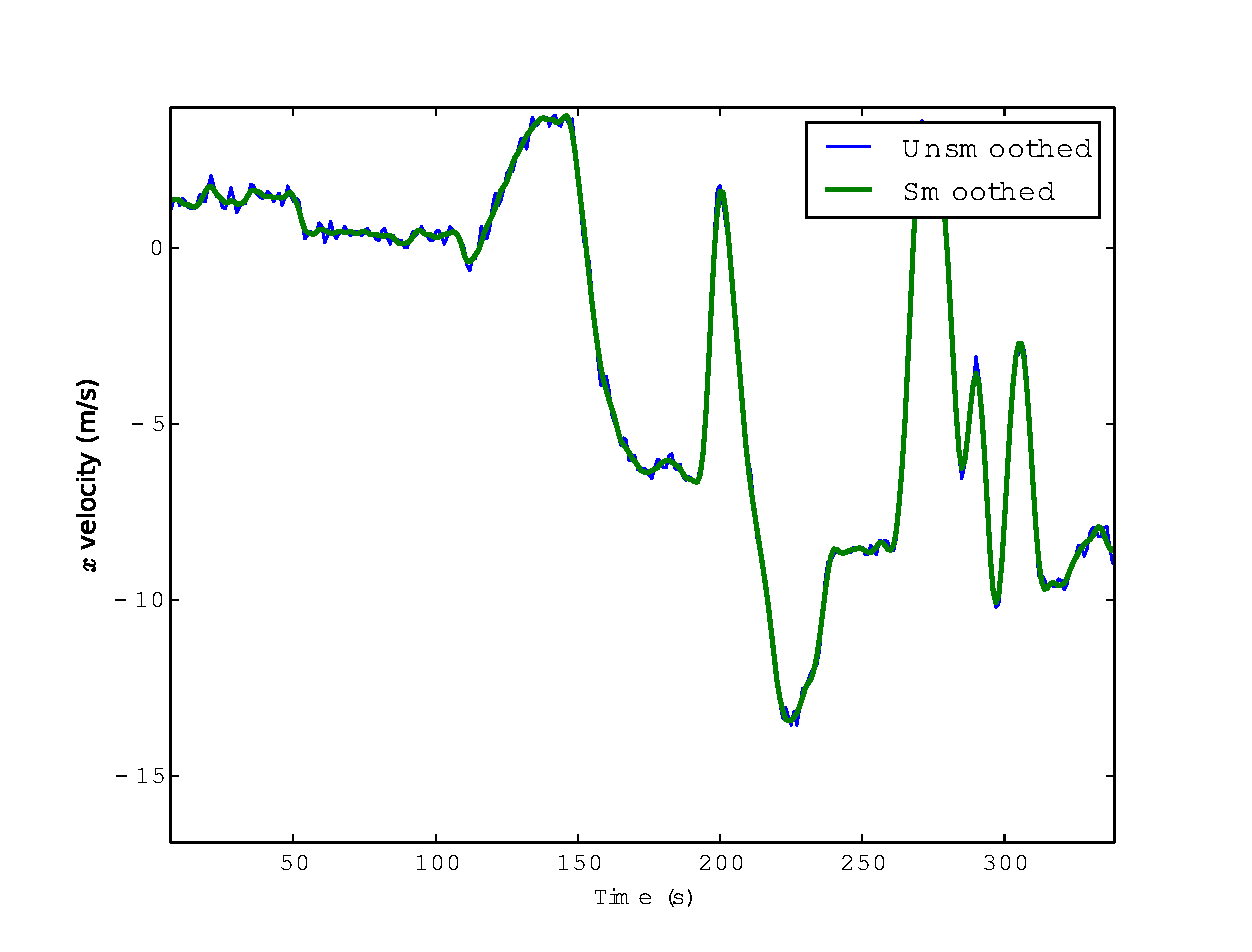
\includegraphics[width=\linewidth]{savgolsmooth}
    \caption{Savitzky-Golay smoothed velocity component.}
    \label{fig:savgolsmooth}
\end{figure}
\subsection{Feature Extraction}
As explained previously, the data does not contain anything that resembles a set of features. So in order to be able to perform machine learning techniques features were first designed and extracted.

\subsubsection{Histogram Features}
A number of different histograms could be taken over speeds, accelerations, acceleration gradient and angular change of the driver. It was hoped that different driving styles would be reflected by differing distributions in these computed measurements. One could also take histograms over combinations of measurements. For example a feature used was a histogram of speed multiplied by angular change. It was hoped that would encapsulate a driver's behaviour whilst he or she made turns. Another feature was a histogram over the cosine of angular change multiplied by speed. Since the cosine of an angle is 1 at zero it was hoped that this histogram would encapsulate a driver's behaviour during straighter sections of road. Additionally histograms were taken when using longer time periods, particularly with angular change which was typically very small over the one second intervals.

\subsubsection{Corner Features}
Other features explored were those associated with corners. It was theorised that the number of corners may characterise the type of route a driver would take. For example a driver that prefers to take back roads may encounter more corners than a driver who prefers main roads. Before such features could be extracted the corners had to first be identified. Algorithm \ref{alg:corners} shows the procedure used for identifying corners. $C$ is a set of corners which is iteratively added to. Vector $\mathbf{v^{(i)}}$ refers to the $ith$ velocity in a trip. The algorithm cycles through the velocity vectors keeping a cumulative sum of distance. If the cumulative distance exceeds a certain value or the angle between the initial velocity and the current velocity is no longer increasing, a check is then made to see if the angle between the current velocity and the initial velocity is above some threshold. If it is a corner has been identified and the process is repeated from after the corner. Otherwise the process is repeated again from one place in front of the start of the current search.

\begin{algorithm}
\begin{algorithmic}
    \State $C \gets \{\}$
    \While{$i < m$}
        \State $d \gets ||\mathbf{v}^{(i)}||_2$
        \If{$d < 1$}
            \State \textbf{continue}
        \EndIf
        \State $j \gets i + 1$
        \State $d_{\text{curr}} \gets d$    
        \State $c_{\text{prev}} \gets 0$ 
        \Loop
            \State{$c_{\text{curr}} \gets \text{angle}(\mathbf{v}^{(i)}, \mathbf{v}^{(j)})$}
            \If{$d_{\text{curr}} > d_{\text{thresh}} \textbf{ or } c_{\text{curr}} < c_{\text{prev}} $ }
                \If{$c_{\text{curr}} > c_{\text{thresh}}$}
                    \State $C \gets C \cup \{(i, j)\}$
                    \State $i \gets j$
                \EndIf
                \State \textbf{break}
            \EndIf
            \State $c_{\text{prev}} \gets c_{\text{curr}}$ 
            \State $j \gets j+1$
        \EndLoop
        \State $i \gets i+1$
    \EndWhile
\end{algorithmic}
\caption{Identifying corners}
\label{alg:corners}
\end{algorithm}

A check is also made to ensure that the vehicle is traveling at a reasonable speed otherwise random fluctuations (even with smoothing) cause problems for the algorithm.

Figure \ref{fig:corners} demonstrates the effectiveness of the algorithm \ref{alg:corners} by showing a trip with the corners found by the procedure highlighted in red. 

\begin{figure}[h]
    \center
    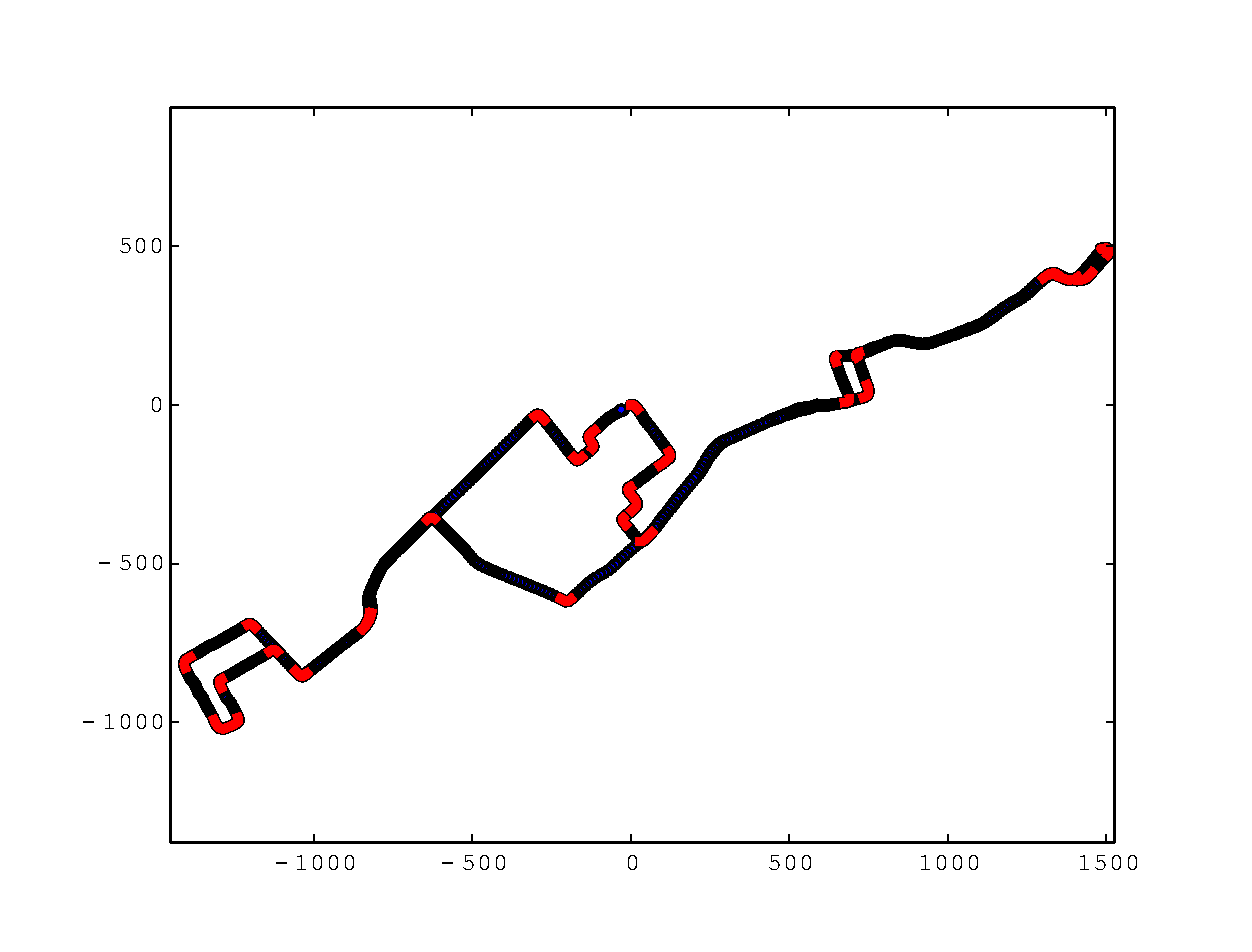
\includegraphics[width=\linewidth]{corners}
    \caption{Plot showing trip with corners highlighted in red.}
    \label{fig:corners}
\end{figure}


\subsubsection{Distance, Velocity \& Time-Related Features}

\begin{figure}[h]
    \center
    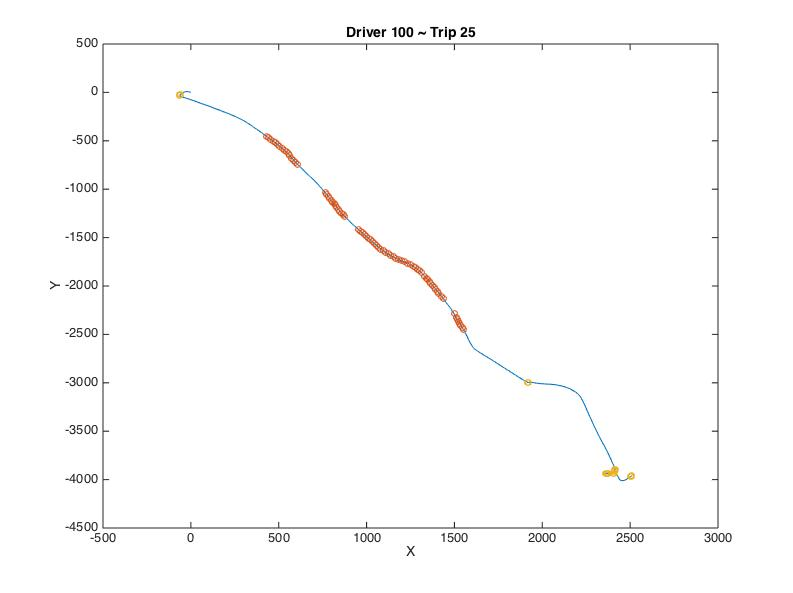
\includegraphics[width=\linewidth]{speed_highlights}
    \caption{Points when the driver is stationary (black) and with low (red) and high (red) velocities.}
    \label{fig:speedpoints}
\end{figure}

% more on distance-related features

A subset of the full set of features (Appendix X) corresponds to distance, speed and time related attributes of trips.
A randomly sampled trip from the dataset is plotted in figure \ref{fig:speedpoints} with coloured points indicating areas of stationary periods (black) and low (yellow) and high (red) velocities.
The thresholds determining ``high" and ``low" velocities were manually configured to best represent the natural motion of a driver along a trip.

% more on speed and time related features



\subsection{Machine Learning}
Whilst the problem scenario prescribes an unsupervised learning technique one can also leverage the fact that the data is labelled. And although the problem is such that some of the data points are mislabelled, supervised learning techniques can still be applied in the hope that the models learned will be general enough such that the mislabelled examples don't affect predictions much. As such a number of different supervised and unsupervised approaches were used in an attempt to solve the problem.


\subsubsection{Supervised Learning Approaches}
For each driver a machine is trained on 180 of their trips labelled as 1 and 180 trips selected from 18 other drivers selected at random each labelled as 0. This process is repeated 10 times such that all trips for that driver have a prediction made on them.

\subsubsection{Gradient Boosting Trees}
Gradient boosting is a technique for combining many weak learning machines into a single machine which achieves better performance. First outlined by Freidman \cite{friedman2001greedy} this proved to be one of the more successful techniques for making predictions based upon the data.



\subsection{Deep Learning}

While many of the common approaches have demonstrated sufficient performance tackling, machine learning, statistical and prediction-based problems, more recent but advanced methods in the field of \textit{deep learning} have attracted much attention due to their vastly clever architectures and training algorithms.
The field started to gain traction when Geoff Hinton \cite{hinton2006fast} released a paper on the discovery of a new training algorithm for deep belief networks.

Deep learning architectures aim to model the structure of the mammal brain, organised in multiple, deep levels \cite{serre2007quantitative}.
In the context of image perception, the primary visual cortex serves to extract local features from scenes or images in the form of bars, edges or lines, then build higher level encodings that compute more precise details about the objects being observed \cite{lee1998role}.
Deep learning tackles the problem of learning representations using this neurologically inspired mechanism by providing a distributed description of its input in a hierarchical structure of progressively more abstract representations.

A typical deep learning model takes the form of a conventional feedforward neural network with many hidden layers and a deep architecture.
However, the term `deep' does not signify the property of a model having many layers but rather the training algorithms used to learn a model in the manner of stacking visible and hidden layers.
Depending on the type of architecture, models may be \textit{over-complete} (more hidden nodes than visible nodes), or \textit{under-complete} (more visible nodes than hidden nodes).
It has been shown that over-complete representations with appropriate regularisation lead to better performing models \cite{vincent2010stacked}.

To assess the performance of deep learning on our problem, a \textit{Deep Belief Network} (DBN) was trained with the features extracted at the preprocessing stage.
A DBN comprises a series of stacked \textit{Restricted Boltzmann Machines} (RBMs).
An RBM is a probabilistic graphical model of connected nodes, or more specifically, an energy-based model of variables (or nodes) $\mathbf{x}$ where the energy of the graph is of the form $p(\mathbf{x})=e^{\mathbf{-E(x)}}$, where $\mathbf{E}$ is an energy function.
An RBM has two layers -- a visible layer and hidden layer.
The objective is to minimise the energy of the model with respect to the weights between the layers.
The training algorithm used is called (one-step) \textit{contrastive divergence} \cite{hinton2002training} and works by sampling between the layers so that the hidden layer learns the visible layer at a different dimension while capturing essential information.
After training an RBM, another can be stacked on top by using the previous hidden layer as the visible layer for the next RBM.

To build a DBN, three RBMs were trained an `unfolded' into a feedforward neural network with one output node representing the binary decision value of whether a trip belongs to the driver.
Each driver was represented by a model specified by the parameters in tables~\ref{table:dbnparams} and~\ref{table:dbnlayers}.

\begin{table}[h]
\centering
\small{
\caption{DBN Parameter Settings}
\label{table:dbnparams}
\begin{tabular}{|l|l|} \hline
\textbf{Parameter}&\textbf{Value}\\ \hline
Activation function & Sigmoid\\ \hline
Batch size & 50\\ \hline
Momentum & 0\\ \hline
Alpha & 1\\ \hline
Training epochs & 5\\ \hline
Model epochs & 50\\ \hline
No. Workers & 16\\ \hline
\end{tabular}}
\end{table}


\begin{table}[h]
\centering
\small{
\caption{DBN Layers}
\label{table:dbnlayers}
\begin{tabular}{|l|l|} \hline
\textbf{Layer}&\textbf{No. nodes}\\ \hline
Input & $N_F$\\ \hline
Hidden & 250\\ \hline
Hidden & 250\\ \hline
Hidden & 250\\ \hline
Output & 1\\ \hline
\end{tabular}}
\end{table}


\subsection{Validation}

\subsection{Large Scale Implementation}

Processing large amounts of data presented many issues and we found the frequency of feedback hindered by the scale of the dataset.
Thus, in order train our models in reasonable time, only a small sample of 200 drivers was used.



% section
\section{Conclusion}

\subsection{Further Work}










\begin{appendices}

\chapter{Features}

\begin{itemize} \itemsep0.5pt \parskip0pt \parsep0pt \ttfamily \small \bfseries
  \item[] first item
  \item[] second item
\end{itemize}

\end{appendices}

\printbibliography
\end{document}
